%!TEX root = ../Thesis.tex
\chapter{Inertial Navigation}

\textit{This chapter describes inertial navigation, as well as how the  together in sensor fusion provide navigation data. Here is documented the work on calibrating the sensor, types of errors encountered.}

\section{Investigations of inertial navigation}
 
Inertial navigation uses measurements by processing signals from accelerometers and gyroscopes to track the position and orientation of an object \cite{UCAM-CL-TR-696}. Navigation is an important part of controlled flight and due to errors being observed in previous rocket flights, particularly in the gyro, as it was observed that if drifts in flight. The intention in this chapter is to study and understand most sources of errors (bias, drift, etc.) that can be encountered in inertial navigation and methods for compensation. 
 
Project requirements state the need for investigating methods of providing  absolute heading (yaw) measurements to correct gyro drift. 
Another requirement is representing navigation attitude through a method that avoids singularities. 
Another requirement was investigating sources of errors in the inertial sensor, particularly the gyro drift in flight.
The final requirement was to investigate filters fit for lower processing power, Arduino class micro controllers. These requirements will be addressed in this chapter. 

\section{Rotation representation}
 
In order to fulfill the requirement concerning rotation representation, three rotation parametrizations have been considered: Euler angles, rotation matrices and quaternions. Out of the aforementioned, quaternions are chosen as the preferred method. Quaternions have the advantage of avoiding both the pitfalls of singularity of Euler angles \cite{4104344} and the overparametrization of rotation matrices, of nine numbers to represent rotation which, in some circumstances, would run into gimbal lock \cite{desrochers2012intelligent}.

\begin{equation}\label{Quaternions}
	\textbf q = q_0 + q_1\textbf{i} + q_2\textbf{j} + q_3\textbf{k} 
\end{equation}

A quaternion (\ref{Quaternions}) is a hyper complex number of rank 4. $ {q_0} $ is the scalar part of the quaternion, with the other three units representing the vectors in ${i j k} $  \cite{fresk2013full}. The navigation calculations will be done by the algorithms in quaternions. Since the quaternion  is  a  complex  number \cite{fresk2013full}, for readability, the output data will be converted from quaternions into Euler angles to facilitate translation and intuitive understanding of the result.

\section{Heading}
 
The system requires a drift-free or absolute heading output, which requires a constant reference point to measure against. Gyro and accelerometer, used so far in flights, provide relative heading and are insufficient for the purpose due to their lack of absolute input for the yaw (heading). With relative heading, the output can drift over time, which reduces accuracy. Having an absolute heading can help solve the gyro drift problem. There are a few choices for absolute heading: sun sensor, star trackers, horizon tracker, cameras, GPS, compass (magnetometer) \cite{hu2015fundamental} - out of these, the most suitable and readily available was the magnetometer. The magnetometer has the advantage of being a lightweight, low power vector sensor, measuring magnitude and direction of the magnetic field (Wertz, 2012, p. 180) \cite{wertz2012spacecraft}. GPS could have been a solution, however, here it is not to be considered for input due to previous reported experience of the GPS not maintaining fix in flight, therefore its data not being usable. 
 
The final decision to solve absolute heading demand is to use a magnetometer, specifically a 9 DoF IMU as opposed to a discrete device. This is because the magnetometer is already available in the current and past IMUs used in the rocket flights - however, it was not used before in navigation data for these reasons: it was difficult to calibrate against the metal launch platform and the metal in the components, as well as being unclear which are the factors influencing magnetometer readings to be calibrated against.Despite challenges, it presents the most accessible option and viable option. The goal in this chapter is to investigate its sources of distortion, as well as methods to counter them. For the purpose of fulfilling the next requirement of examining sources of errors in the inertial navigation, the inertial sensor will be examined, along with its characteristic measurement disturbances. 
 
\section{The Inertial Measurement Unit sensor} 
 
Inertial measurement units (IMU) typically contain three orthogonal rate-gyroscopes and three orthogonal accelerometers, measuring angular velocity and linear acceleration.  \cite{UCAM-CL-TR-696}, while a MARG system (Magnetic, Angular Rate, and Gravity) is an IMU with added magnetometer.The  IMU is restricted to outputting orientation measurements relative to the direction of gravity, whereas MARG systems provide orientation relative to the direction of gravity and the earth's magnetic field \cite{madgwick2010efficient}. For simplicity, the sensors used is referred to as IMU throughout this project, despite it being a MARG system. Thus, the sensors used in this project were MEMS (microelectromechanical system) IMU consisting of tri-axis: 
 
\begin{itemize}
\item Accelerometer
\item Gyroscope
\item Magnetometer
\end{itemize}

The accelerometer measures the external specific force acting on the sensor, consisting on both the sensor’s acceleration and gravity \cite{kok2017using}. The gyroscope measures the sensor's angular velocity, that is, the rate of change of the sensor's orientation, in the body frame. Magnetometer measures the earth’s magnetic field.  
 
\section{IMU sensor errors} 

Accurate acceleration, angular rate and magnetic field measurements are essential for sensor fusion algorithms and the correct estimation of orientation. It has been noted that without error compensation, the devices experience significant distortions; the gyroscope, in particular, has a drift of 5-15 degrees/minute  \cite{barshan1995inertial}, but with proper error calibration, the output measurements can be significantly improved. For that purpose, common types of errors occurring in a MARG device will be investigated, as well as methods of compensation for such errors. 

\textbf{Accelerometer distortions} consist of: noise, undesired high frequency oscillations; bias (offset), deviation from ideal output and vibration, read by the sensor as linear acceleration, adding to the high frequency noise. Thus, the accelerometer sensor model is described as:

\begin{equation}\label{accmodel}
	{a}(t)={a_b}(t)+g+b_{acc}(t)+n_{acc}(t)
\end{equation}

where: ${a}(t) $ is the acceleration reported by the sensor, $ a_b $ is the true acceleration of the body, $g$ is the gravitational acceleration, $b_{acc}(t)$ is the offset (bias) of the sensor and $n_{acc}(t)$ is the signal noise.


\textbf{Gyroscope distortions} are its bias (offset), deviation from ideal output
and random drift (walk), observed in the output deviation over time due to disturbances in the sensor \cite{lawrence1998gyro}. Therefore, the Sensor gyro model is described by the equation:

\begin{equation}\label{gyromodel}
	{\omega}(t)={\omega_b}(t)+b_{gyro}(t)+n_{gyro}(t)
\end{equation}

where: ${\omega}(t) $ is the angular rate reported by the sensor, $ {\omega_b} $ is the true angular rate  of the body, $b_{gyro}(t)$ is the bias of the sensor and $n_{gyro}(t)$ is the signal noise (drift). \cite{euston2008complementary}

\textbf{Magnetometer distortions} are: hard offset, strong effects caused by manufacturing defects in the sensor or environment distorsions; soft offset, produced by less pronounced magnetic objects in the sensor’s environment which distort the surrounding magnetic field; and magnetic declination, the position of the magnetic north relative to the geographic north, depending on location coordinates. Following, the magnetometer sensor model described as:

 \begin{equation}\label{magmodel}
	{m}(t)={m_b}(t)+b_{m}(t)+n_{m}(t)+d_m
\end{equation}
 
 where: ${m}(t) $ is the magnetic field measurement reported by the sensor, $ {m_b} $ is the true magnetic field measurement of the body, $b_{m}(t)$ is the offset (bias) of the sensor, hard iron distortion in the case of the magnetometer and $n_{m}(t)$ is the signal noise. $ d_m$ is the magnetic declination, dependant on location. 

Cross-coupling has been observed particularly in the lower quality IMUs, meaning some data was passed between axes of the same device (X readings read in Y) or accelerometer sending readings to the gyro (vibration being picked by the gyro, a clear error, as vibration is linear acceleration which should only be measured by the accelerometer).
 
\section{IMU calibration process}

Due to sensor readings distortions, pre-processing is required in order for the measurements to provide useful estimation. The calibration and alignment process has followed the same steps for each IMU device tested in this project. One of the components, usually the magnetometer, has a different set of axes and reference frame than the others and so the axes need to be consulted after reading the datasheet and the output data in order to find the reference frame and align them accordingly. 
 
\begin{figure}[h!]
  \centering
  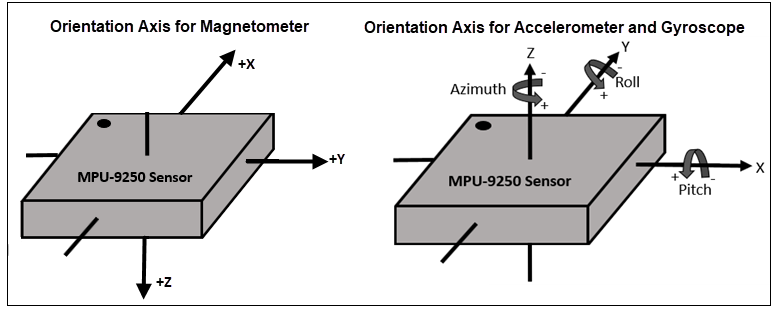
\includegraphics[scale=0.8]{graphics/mpu9250.png}
  \caption{Axes difference on accelerometer-gyro and magnetometer}
  \label{fig:mpu}
\end{figure} 
 

In this project, the linear axes were defined as positive NED (north, east, down), and the rotational (gyro) as positive counterclockwise. Depending on the IMU and the chosen frame of reference, the accelerometer and the gyroscope axes will be swapped and/or inverted to match the magnetometer axes. For example, in the case of the MPU-9250 (figure \ref{fig:mpu}), in order to align to NED convention, the the x and y axes of the accelerometer-gyro were swapped and the z axis was inverted, which is in alignment with the existing axes of the magnetometer device. 


Then it is necessary to determine polarity values for the accelerometer, and gyroscope, by reading their data and determining which is the positive and negative direction of each axis. The accelerometer polarity can be determined by reading the gravity values, whether positive or negative. The gyroscope readings display whether clockwise or counterclockwise positive for each axis and can be inverted in case of non-alignment with the chosen convention, in this case, counterclockwise positive. The rotation axes were defined as \cite{de2012spacecraft}: roll is the rotation about the x axis, pitch is the rotation about the y axis, yaw is the rotation about the z axis. 

Calibration of the sensor is important before fusing, filtering and using the output. The calibration process of the accelerometer, gyroscope and magnetometer has some similarities, in the sense that all three require the removal of offsets (biases); then the noise, drift, and vibration characteristic to each component is handled by the sensor fusion filters chosen, described below. 

\textbf{Accelerometer} offsets are removed by reading the gravity vector in each axis while on a flat surface and compensating accordingly until the reading shows 9.8 or 1g, depending on the chosen unit of measurement. \textbf{Gyroscope} bias is removed in a similar fashion, by what is known as the tombstone test, where the sensor is placed flat on a surface, and compensations are applied to level the values to 0. \textbf{Magnetometer} is affected by hard iron effects, causing deviation from origin and soft iron offsets, causing skew, stretching the magnetic sphere towards an ellipse shape. In order to determine the offsets, the magnetometer must be moved in a eight-shape or to cover as many orientations as possible during the measurements, to fully capture environment distortion. Figure \ref{fig:Magnetometer} shows the deviation caused by hard iron effects and the ideal sphere that represents calibrated magnetometer data. 
 
 \begin{figure}[H]
  \centering
  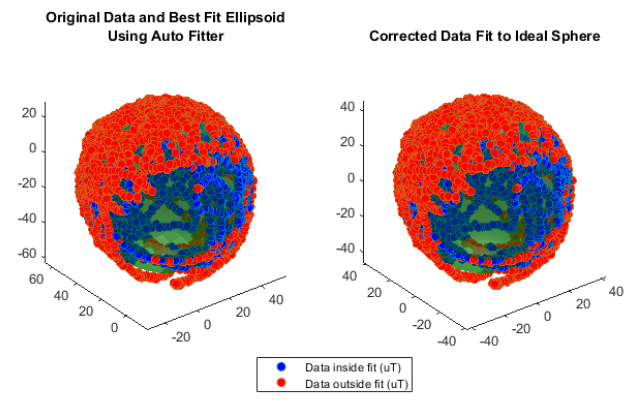
\includegraphics[scale=0.7]{graphics/mag.png}
  \caption{Magnetometer samples fit to ideal sphere}
  \label{fig:Magnetometer}
\end{figure}
 
 Figure \ref{fig:mag_uncalibrated} shows the measurements from figure \ref{fig:Magnetometer}, as example of hard offset calibration, with  little noticeable skew from soft iron effects. 
  
\begin{figure}[H]
    \centering
    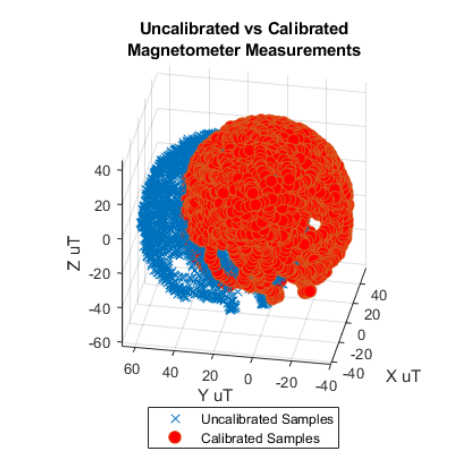
\includegraphics[scale=0.7]{graphics/mag0.png}
    \caption{Hard offset effects calibration}
     \label{fig:mag_uncalibrated}
\end{figure}
 
 
This process has been performed on each IMU tested. Figures \ref{fig:mag__very_uncalibrated}, \ref{fig:mag_uncalibrated} and \ref{fig:Magnetometer} show data collected from an IMU during calibration process. In figure \ref{fig:mag__very_uncalibrated}, hard iron the offset can be observed in the uncalibrated readings by the deviation from (0,0,0) origin; the soft iron effect can be noticed in the ellipsoid shape of the samples, as opposed to a spherical shape, expected in the case of calibrated data. 

\begin{figure}[H]
 \centering
 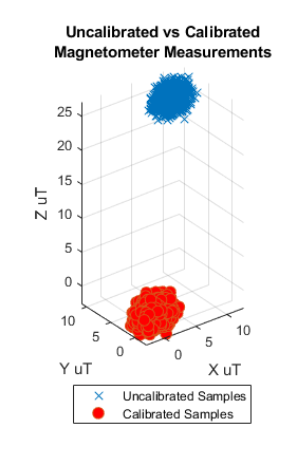
\includegraphics{graphics/magoff.png}
  \caption{Strong effects of hard iron and soft iron distortions in uncalibrated magnetometer measurements vs hard iron calibrated measurements}
  \label{fig:mag__very_uncalibrated}
\end{figure}

These figures have covered the cases of offset distortion in magnetometer readings. The last distortion experienced by the magnetometer, magnetic declination, is to be determined based on location - in Copenhagen, Denmark, the declination is +4.37°, which is added as a correction to the heading readings. Since the magnetometer picks up magnetic fields, any slight change in the environment requires a new calibration. 

 \section{Sensor fusion}
 
 The calibrated measurements of the sensor are not directly usable, due to sensor noise, picking up vibration or other mechanical disturbances even when static. \cite{patonis2018fusion}
 After calibration of the sensor, the measurements can be combined through sensor filtering to produce more accurate, usable estimation of position and orientation. The main consideration for choosing filters has been their efficiency and computational cost.  
 
The following filters have been tested in this project:
 
\begin{itemize}
\item Integrated gyro measurements
\item Complementary
\item Mahony
\item Madgwick
\end{itemize}

The first solution is having the gyroscope angular rate integrated over time in order to obtain angular position, acting as a high-pass filter.
The complementary filter is a common, fast, efficient solution for inertial measurements. It acts by low-pass filtering accelerometer data, and high-pass filtering by direct integration of gyroscope data, then fusing  these estimates together \cite{euston2008complementary}. 
It uses the fact that the measurements from accelerometer and magnetometer are noisy yet steady over time, while gyroscope measurements are accurate in short periods, but drift over time. It results that in frequency domain, the gyroscope has desirable properties at high frequencies, therefore it requires a high-pass filter; while accelerometer and magnetometer have useful properties at low frequencies, which can be exploited through a low-pass filter.  \cite{kok2017using}. By combining the advantages of each group, they complement for each other's deficiencies. However, the Euler angles calculated from the complementary filter and integrating gyro data are prone to singularities. 

The following two are quaternion-based filters. 
Mahony or Explicit Complementary Filter, is a non-linear complementary filter, designed specifically for low-cost inertial measurement units and capable of achieving the same results as an extended Kalman filter with GPS and inertial data. This filter has been validated only for inertial data from accelerometer-gyro. \cite{euston2008complementary}
Madgwick filter has been proven to produce similar to \cite{cirillo2016comparison} or improved accuracy over Kalman-based algorithms \cite{madgwick2010efficient}, with the advantage of having low computation cost, suitable for Arduino class micro-controllers. Another advantage over Mahony filter is its suitability for IMU and MARG systems, therefore, including magnetometers.

Madgwick filter has a tunable parameter, $\beta$, related to the gyroscope measurement error. A lower value for the parameter will decrease the influence of the accelerometer and magnetometer, allowing the gyroscope measurements to have a higher weight\cite{madgwick2010efficient}. This project uses the library implementation of \cite{SensorFusion} for Mahony and Madgwick filters. There was testing with the value of $\beta$ for Madgwick, initially tested with 0.1 and with values ranging to 0.9. The best outcome was found with the value of 0.5, as it converges quicker than having lower values and it balances the drift from the gyroscope. However, this is assuming usable, calibrated measurements from the accelerometer and magnetometer.

\section{Hardware used: IMU and Arduino}

There have been several IMUs tried over the course of this project, from the least quality to highest:
 
\begin{itemize}
\item GY-521 
\item MPU6050
\item Razor 9 DoF
\item LSM9DS1
\item BNO055 
\end{itemize}


First two IMUs were 6 DoF (accelerometer and gyro), without magnetometer, which was insufficient for the purpose of project after deciding on magnetometer as absolute heading sensor. In addition, their gyroscopes were picking up vibration, which signifies axes and device cross-talk - an error, as the gyro should not pick up vibration, since it is linear acceleration. Next two devices were 9 DoF sensors, with different challenges due to their magnetometer in particular. However, the primary challenge was they turned out overall unsuitable for aerial devices, as the noise was significant, it required extensive calibration and filtering, which introduced serious delays. The final choice was BNO055, which proved to be the most reliable device out of the list and suitable for the purpose.
 
\begin{figure}[H]
    \centering
    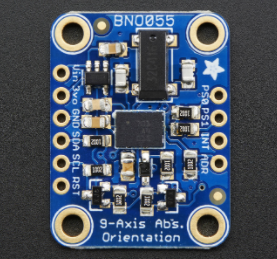
\includegraphics[scale=0.8]{graphics/BNO055.png}
    \caption{BNO055 IMU sensor}
     \label{fig:mag_uncalibrated}
\end{figure} 
 
 
Several Arduino class microcontrollers were used, due to their different capabilities: Mega, Uno, Nano, as well as a variant of Nano with SAMD21 processor. The processing power of the Nano, atm328, turned out to be insufficient for the Madgwick filter so the original Nano was replaced it with a SAMD21 processor version of the Nano. The final code was settled on Nano/SAMD21 because of the superior processor, smaller size, made with code for Madgwick/Mahony/complementary filter plus a PID controller. However, since there was intent to use Simulink, which does not support the Nano/SAMD21, another Arduino Mega is used for the code generated from Simulink. 
 
 \textit{This chapter discussed the different types of challenges met in inertial navigation, for the purpose of investigating and finding ways of countering them to ensure accurate navigation. 
The next chapters will discuss the modelling and control of the system.}



